\subsection{\texorpdfstring{应用：I. \(L^{p}\) 空间的对偶}{应用：I. L to the p 空间的对偶}}

我们在这里只处理实空间 \(\mathbf{L}^p\) 的情形。

回忆一下，两个数 \(p, q\) （满足 \(1 \leqslant p \leqslant +\infty\) ，\(1 \leqslant q \leqslant +\infty\) ，\(1/p + 1/q = 1\) 者）称为共轭指数（Ch. IV, §6, No.~4）。每个函数 \(g \in \mathcal{L}^q\) 定义一个连续线性形式 \(\theta_g\) （\(L to the p\) 上的），它是由线性形式 \(f \mapsto \int fg d\mu\) （\(\mathcal{L}^p\) 上的）出发过渡到商而得到的，并且有 \(N_q(g) = \| \theta_g \|\) （Ch. IV, §6, No.~4, 命题 3 的推论）。通过过渡到商，我们就从映射 \(g \mapsto \theta_g\) 得到一个等距线性映射 \(\varphi\) ，把 \(L^q\) 映入对偶 \((L to the p)'\) （\(L to the p\) 的）。我们将证明，对 \(1 \leqslant p < +\infty\) ，\(\varphi\) 把 \(L^q\) 映到 \((L to the p)'\) 上，因而今后我们可以把 Banach 空间 \(L^q\) 与 Banach 空间 \((L to the p)'\) 借助同构 \(\varphi\) 等同起来。用另一种方式陈述：

定理 4. --- 设 p 和 q 是满足 \(1 \leqslant p < +\infty\) 的两个共轭指数。\(\mathcal{L}^{p}(\mathrm{T}, \mu)\) 上的每个连续线性形式都是 \(f \mapsto \int fg d\mu\) 型的，其中 g 是 \(\mathcal{L}^{q}(\mathrm{T}, \mu)\) 中的一个函数，它的类在 \(L^{q}\) 中是适定的。

设 \(\theta\) 是 \(\mathcal{L}^p\) 上的一个连续线性形式；于是，存在一个数 \(a \geqslant 0\) ，使得 \(|\theta(f)| \leqslant a \cdot \mathrm{N}_p(f)\) 对每个函数 \(f \in \mathcal{L}^p\) 成立。考察 \(\theta\) 在具有紧支集的连续函数所组成的空间 \(\mathcal{K}(\mathrm{T})\) 上的限制：对 T 的每个紧子集 K 以及每个函数 \(f \in \mathcal{K}(\mathrm{T}, \mathrm{K})\) （支集含于 K 中的连续函数所组成的空间），有 \(\mathrm{N}_p(f) \leqslant (\mu(\mathrm{K}))^{1/p} \| f \|\) ；因此在 \(\mathcal{K}(\mathrm{T}, \mathrm{K})\) 上由 \(\mathcal{L}^p\) 的拓扑诱导的拓扑比一致收敛拓扑粗，从而 \(\theta\) 在每个 \(\mathcal{K}(\mathrm{T}, \mathrm{K})\) 上的限制对后一拓扑是连续的。这意味着 \(\theta\) 在 \(\mathcal{K}(\mathrm{T})\) 上的限制是一个实测度 \(\nu\) （Ch. III, §1, No.~3, 定义 2）。

我们来证明 \(|\nu|(|f|) \leqslant a \cdot \mathrm{N}_{p}(f)\) 对 \(\mathcal{K}(\mathrm{T})\) 中的每个函数 f 成立。只须对 \(f \geqslant 0\) 证明此公式。现在，对每个函数 \(\psi\) （\(\mathcal{K}(\mathrm{T})\) 中满足 \(|\psi| \leqslant f\) 者），我们有

\[
| \nu (\psi) | \leqslant a \cdot \mathrm{N} _ {p} (\psi) \leqslant a \cdot \mathrm{N} _ {p} (f);
\]

我们的断言由 Ch. III, §1, No.~6 公式 (12) 给出的测度绝对值的表达式得出。关系 \(|\nu|(|f|) \leqslant a(\mu(|f|^p))^{1/p}\) 通过过渡到下包络，立即推广到 \(f\) 是一个紧集的特征函数的情形，然后它蕴涵每个 \(\mu\) -可忽略的紧集都是 \(\nu\) -可忽略的，从而 \(\nu\) 是一个以 \(\mu\) 为基的测度（No.~5, 定理 2）。

于是，存在一个局部 \(\mu\) -可积的正函数 \(h_1\) ，使得 \(|\nu|(f) = \int fh_1 d\mu\) 对每个函数 \(f \in \mathcal{K}(\mathrm{T})\) 成立。我们来证明，\(h_1\) 局部几乎处处等于 \(\mathcal{L}^q\) 中的一个函数。若函数 \(f \geqslant 0\) 属于 \(\mathcal{K}(\mathrm{T})\) 且满足 \(\mathrm{N}_p(f) \leqslant 1\) ，则 \(\int fh_1 d\mu = |\nu|(f) \leqslant a\) 。对每个连续映射 \(f_0\) （由 \(\mathrm{T}\) 到 {[}0,1{]} 中且具有紧支集的），我们因此有 \(\sup \int (f_0 h_1) f d\mu \leqslant a\) ，其中 \(f\) 跑遍函数 \(\geqslant 0\) （\(\mathcal{K}(\mathrm{T})\) 中满足 \(\mathrm{N}_p(f) \leqslant 1\) 者）所成之集。由此，借助 Chap. IV, §6, No.~4 的公式 (11)，可以推出 \(\mathrm{N}_q(f_0 h_1) \leqslant a\) 。从而 \(\sup_{\mathrm{K}} \mathrm{N}_q (\varphi_{\mathrm{K}} h_1) \leqslant a\) ，其中 \(\mathrm{K}\) 跑遍 \(\mathrm{T}\) 的紧子集所成之集，这就证明了我们的断言（§1, 命题 9）。

设 v 是一个绝对值为 1 的普遍可测（实）函数，使得 \(\nu = v \cdot |\nu|\) （定理 2 的推论 3），并设 \(g = v h_{1}\) ；则 \(\nu = g \cdot \mu\) ，且 g 属于 \(L^{q}\) 。对每个函数 \(f \in \mathcal{K}(T)\) ，我们有 \(\theta(f) = \nu(f) = \int fg d\mu\) 。换言之，连续线性形式 \(\theta\) 和 \(\theta_{g}\) 在 \(\mathcal{K}(T)\) 上一致；因而它们在 \(L^{p}\) 上相等，因为 \(\mathcal{K}(T)\) 在 \(L^{p}\) 中稠密，这就完成了证明。

推论. --- 对满足 \(1 < p < +\infty\) 的每个数 p ，Banach 空间 \(L^{p}(T, \mu)\) 是自反的。

\pandocbounded{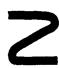
\includegraphics[keepaspectratio]{images/part002_5aba953c.jpg}}

一般地，\(L^{\infty}\) 的对偶不同构于 \(L^{1}\) ，因而 \(L^{1}\) 和 \(L^{\infty}\) 不是自反的（习题 10）。我们来刻画 \(L^{\infty}\) 上由线性形式 \(g \mapsto \int fg d\mu\) （\(L^{\infty}\) 上的，其中 \(g \in L^{1}\) ）过渡到商而产生的那些连续线性形式。

序向量空间 \(\mathrm{L}^{\infty}(\mathrm{T},\mu)\) （它是 \(\mathrm{L}_{\mathrm{loc}}^{1}(\mathrm{T},\mu)\) 的一个子空间）是完全格序的；因为，若 \((f_{\alpha})\) 是 \(L^{\infty}\) 中的正函数的一个族，其类所成之集 \((\dot{f}_{\alpha})\) 在 \(L^{\infty}\) 中有上界，则存在 \(a\geqslant0\) ，使得 \(\mathrm{N}_{\infty}(f_{\alpha})\leqslant a\) 对一切 \(\alpha\) 成立。由于 \(\mathrm{L}_{\mathrm{loc}}^{1}(\mathrm{T},\mu)\) 是完全格序的，族 \((\dot{f}_{\alpha})\) 有一个上确界 \(\dot{h}\) （在 \(\mathrm{L}_{\mathrm{loc}}^{1}(\mathrm{T},\mu)\) 中）；但由于 \(\dot{a}\geqslant\dot{f}_{\alpha}\) 对每个 \(\alpha\) 成立，我们有 \(\dot{h}\leqslant\dot{a}\) ，从而 \(\mathrm{N}_{\infty}(h)\leqslant a\) ，由此得到我们的断言。

命题 14. --- 为使一个正线性形式 \(\theta\) （\(\mathcal{L}^{\infty}\) 上的）是 \(f \mapsto \int fg d\mu\) 型的（其中 \(g \in \mathcal{L}^{1}\) ），必须且只须：对每个递增有向的正函数族 \((f_{\alpha})_{\alpha \in \mathrm{A}}\) （\(\mathcal{L}^{\infty}\) 中的），若其类所成之集 \((\dot{f}_{\alpha})_{\alpha \in \mathrm{A}}\) 在 \(\mathrm{L}^{\infty}\) 中有上界且在此空间中以 \(\dot{h}\) 为上确界，则有

\[
\theta (h) = \sup _ {\alpha \in \mathrm{A}} \theta (f _ {\alpha}).
\]

我们先证明条件是必要的。测度 \(h \cdot \mu\) 在 \(\mathcal{M}(\mathrm{T})\) 中是测度 \(f_{\alpha} \cdot \mu\) 所成之集的上确界（No.~5, 概说）；因此（Ch. II, §2, No.~2），对每个函数 \(\varphi \geqslant 0\) （\(\mathcal{K}(\mathrm{T})\) 中的），我们有 \(\int h\varphi d\mu = \sup_{\alpha \in \mathrm{A}} \int f_{\alpha}\varphi d\mu\) 。现在，若 \(a\) 是一个数 \(\geqslant 0\) ，使得 \(\mathrm{N}_{\infty}(f_{\alpha}) \leqslant a\) 对所有 \(\alpha \in \mathrm{A}\) 成立（这蕴涵 \(\mathrm{N}_{\infty}(h) \leqslant a\) ），则对每个 \(\varepsilon > 0\) ，存在一个 \(\varphi \in \mathcal{K}(\mathrm{T})\) ，满足 \(\varphi \geqslant 0\) 且 \(\mathrm{N}_1(g - \varphi) \leqslant \varepsilon\) ，由此我们推出 \(\int f_{\alpha}|g - \varphi| d\mu \leqslant a\varepsilon\) 对所有 \(\alpha \in \mathrm{A}\) 成立，以及 \(\int h|g - \varphi| d\mu \leqslant a\varepsilon\) 。由于 \(\sup_{\alpha \in \mathrm{A}} \int f_{\alpha}g d\mu \leqslant \int hg d\mu\) ，这就证明了这个不等式的两个成员相等。

为证明条件是充分的，我们将用到下列引理：

引理 4. --- \(1^{\circ}\) 设 \(f\) 是 \(\mathbf{T}\) 上的一个下半连续且有界的正函数。则它的类 \(\dot{f}\) （\(\mathbf{L}^{\infty}\) 中的）是类 \(\dot{\varphi}\) 所成之集的上确界，其中 \(\varphi\) 跑遍 \(\mathcal{K}(\mathbf{T})\) 中满足 \(0 \leqslant \varphi \leqslant f\) 的函数所成之集。

\(2^{\circ}\) 设 \(f\) 是 \(\mathbf{T}\) 上的一个可测且有界的正函数。则它的类 \(\dot{f}\) （\(\mathrm{L}^{\infty}\) 中的）是类 \(\dot{\psi}\) 所成之集的下确界，其中 \(\psi\) 跑遍 \(\mathbf{T}\) 上的下半连续且有界且 \(\geqslant f\) 的函数所成之集。

\(1^{\circ}\) 设 \(f'\) 是 \(\mathcal{L}^{\infty}\) 中的一个函数，使得 \(\dot{f}'\) 在 \(\mathrm{L}^{\infty}\) 中是类 \(\dot{\varphi}\) 所成之集的上确界，其中 \(\varphi\) 跑遍 \(\mathcal{K}(\mathrm{T})\) 中满足 \(0 \leqslant \varphi \leqslant f\) 的函数；显然 \(\dot{f}' \leqslant \dot{f}\) 。设 U 是 T 的一个相对紧开子集；对每个函数 \(h\) （\(\mathcal{K}(\mathrm{T})\) 中满足 \(0 \leqslant h \leqslant f\varphi_{\mathrm{U}}\) 者），依定义有 \(h(t) \leqslant f'(t)\) 局部几乎处处成立，因此 \(h(t) \leqslant f'(t)\varphi_{\mathrm{U}}(t)\) 几乎处处成立；由此推出 \(\int h d\mu \leqslant \int f'\varphi_{\mathrm{U}} d\mu\) 。然而，由于 \(f\varphi_{\mathrm{U}}\) 是下半连续的，有 \(\int f\varphi_{\mathrm{U}} d\mu = \sup \int h d\mu\) ，其中 \(h\) 跑遍 \(\mathcal{K}(\mathrm{T})\) 中满足 \(0 \leqslant h \leqslant f\varphi_{\mathrm{U}}\) 的函数所成之集（Ch. IV, §1, No.~1, 定义 1）；因此

\[
\int f \varphi_ {\mathrm{U}} d \mu \leqslant \int f ^ {\prime} \varphi_ {\mathrm{U}} d \mu ,
\]

而由于 \(f' \varphi_{\mathrm{U}} \leqslant f \varphi_{\mathrm{U}}\) 几乎处处成立，必然有 \(f \varphi_{\mathrm{U}} = f' \varphi_{\mathrm{U}}\) 几乎处处成立，从而 \(f = f'\) 局部几乎处处成立。

\(2^{\circ}\) 设 \(f'\) 是 \(\mathcal{L}^{\infty}\) 中的一个函数，使得 \(\dot{f}'\) 在 \(\mathrm{L}^{\infty}\) 中是由类 \(\dot{\psi}\) （\(\psi\) 为有界且 \(\geqslant f\) 的下半连续函数）组成的集的下确界；则 \(\dot{f}' \geqslant \dot{f}\) 。设 K 是 T 的一个紧子集；对每个下半连续且有界且 \(\geqslant f\varphi_{K}\) 的函数 h ，用 \(\overline{h}\) 表示在 K 上等于 h 且在 T - K 上等于 \(\|f\| + \|h\|\) 的函数。则 \(\overline{h}\) 是下半连续的且 \(\geqslant f\) ，因此依定义 \(\overline{h}(t) \geqslant f'(t)\) 局部几乎处处成立；由此推出 \(h(t) \geqslant f'(t)\varphi_{\mathrm{K}}(t)\) 几乎处处成立，从而 \(\int h d\mu \geqslant \int f'\varphi_{K} d\mu\) 。但 \(\int f\varphi_{K} d\mu = \inf \int h d\mu\) ，其中 h 跑遍下半连续且有界且 \(\geqslant f\varphi_{K}\) 的函数所成之集（Ch. IV, §1, No.~3, 定义 3）；因此

\[
\int f \varphi_ {\mathrm{K}} d \mu \geqslant \int f ^ {\prime} \varphi_ {\mathrm{K}} d \mu ,
\]

而由于 \(f\varphi_{\mathrm{K}} \leqslant f'\varphi_{\mathrm{K}}\) 几乎处处成立，必然有 \(f\varphi_{\mathrm{K}} = f'\varphi_{\mathrm{K}}\) 几乎处处成立，从而 \(f = f'\) 局部几乎处处成立。

引理既已证明，设 \(\theta\) 是 \(\mathcal{L}^{\infty}\) 上满足命题 14 陈述中条件的正线性形式。\(\theta\) 在空间 \(\mathcal{K}(\mathrm{T})\) 上的限制是一个正测度 \(\nu\) （\(\mathrm{T}\) 上的）。我们将证明，对每个正函数 \(f\in \mathcal{L}^{\infty}(\mathrm{T},\mu)\) ，有 \(\theta (f) = \nu^{*}(f)\) 。先设 \(f\) 是下半连续的（且有界）；由引理 4，\(\dot{f}\) 是类 \(\dot{\varphi}\) 的递增有向集的上确界，其中 \(\varphi\) 跑遍有向集 \(\Phi\) （由 \(\mathcal{K}(\mathrm{T})\) 中满足 \(0\leqslant \varphi \leqslant f\) 的函数组成）。由于依假设 \(\theta (f) = \sup_{\varphi \in \Phi}\theta (\varphi)\) ，且依定义 \(\nu^{*}(f) = \sup_{\varphi \in \Phi}\nu (\varphi)\) ，我们的断言在这一情形得证。其次，设 \(f\) 是 \(\mu\) -可测且有界的；则依定义 \(\nu^{*}(f) = \inf_{\psi \in \Psi}\nu^{*}(\psi)\) ，其中 \(\psi\) 跑遍递减有向集 \(\Psi\) （由下半连续且有界且 \(\geqslant f\) 的函数组成）。若 \(a\geqslant \| f\|\) ，则把陈述中的假设应用于函数 \(a - \psi\) （\(\psi \in \Psi\) 且 \(\psi \leqslant a\) 者）的类所组成的递增有向集，即依引理看出 \(\theta (f) = \inf_{\psi \in \Psi}\theta (\psi)\) ，因而确有 \(\theta (f) = \nu^{*}(f)\) 。特别地，对每个 \(\mu\) -可忽略的函数 \(f\geqslant 0\) ，有 \(\theta (f) = 0\) ，因此 \(\nu^{*}(f) = 0\) ，从而（No.~5, 定理 2）\(\nu\) 是一个以 \(\mu\) 为基的测度；此外，\(\nu^{*}(1) = \theta (1) < +\infty\) ，因而（定理 1 的推论）\(\nu = g\cdot \mu\) ，其中 \(g\in \mathcal{L}^1 (\mathrm{T},\mu)\) 。最后，由于每个 \(\mu\) -可测函数都是 \(\nu\) -可测的，每个正函数 \(f\in \mathcal{L}^{\infty}(\mathrm{T},\mu)\) 都是 \(\nu\) -可积的，且 \(\int fg d\mu = \nu^{*}(f) = \theta (f)\) ，这就完成了证明。

由命题 14 可以得出，\(\mathcal{L}^{\infty}\) 上 \(f\mapsto \int fg d\mu\) 型（其中 \(g\in \mathcal{L}^{1}\) ）的线性形式就是差 \(\theta_{1} - \theta_{2}\) ，其中 \(\theta_{1}\) 和 \(\theta_{2}\) 是满足命题 14 的条件的正线性形式。

